\section{Ideas for New Alternative Games}
\label{chap:new_ideas}

In this chapter, a description and evaluation of six alternative game concepts invented during our prestudy work will be presented. Previously (in Chapter \ref{chap:what_is_alternative_game}), we have defined and constructed a model to establish what an alternative game is. The model was used to develop new ideas, as illustrated in Figure \ref{fig:new_ideas_process}. Starting with a loose idea and then tweaking the characteristics made us invent new concepts that we otherwise would not have considered. This process is a generalized approach that can generate alternative games from ideas that are initially regular games or as an iterative process to add more alternative features.

\begin{figure}[H]
    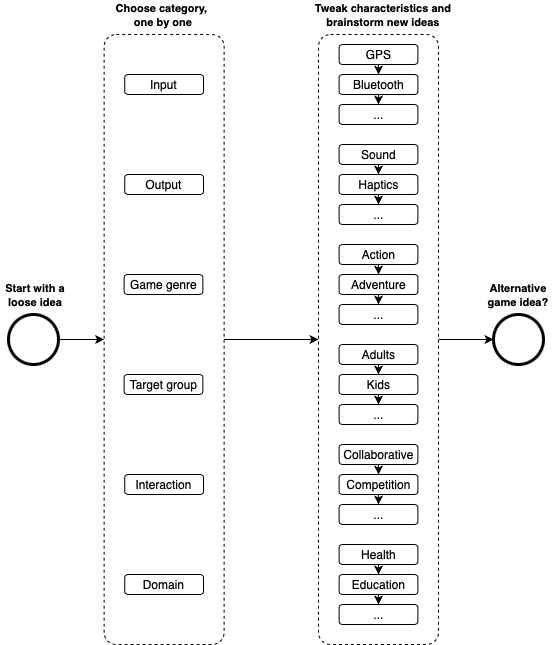
\includegraphics[width=0.60\textwidth]{Images/NewIdeas/NewIdeasProcess.png}
    \centering
    \caption{Inventing new ideas with our alternative games model}
    \label{fig:new_ideas_process}
\end{figure}

Later, we studied literature explaining how to create an enjoyable game, reward systems, and player types in chapters \ref{chap:design_an_enjoyable_game}, \ref{chap:reward_systems}, and \ref{chap:player_types}. The knowledge obtained from this work gave us insight into game design. Finally, Chapter \ref{chap:existing_games} gave us an overview of existing alternative games. This research showed us examples of the current possibilities and stimulated our fantasy to invent even more ideas.

After outlining and evaluating the six ideas, the model defined in our prestudy will be used to compare them. This comparison will, similar to Chapter \ref{chap:existing_games}, help us describe the differences between the games and why they characterize as alternative.

Our primary motivation for choosing this specific task was the opportunity to create an application with a socially beneficial purpose. The concepts should preferably introduce something valuable to society while still exploring the genre of alternative games. Also, the goal was to make the application available to as many users as possible. Based on these factors, we decided early that the game had to be based on the mobile platform. Consequently, the concepts described later in this chapter are invented with this in mind. Over three billion people own a smartphone today \citep{odea_smartphone_2020}. By targeting the smartphone market and these two operating systems, we can reach many potential users. Furthermore, smartphones have a variety of sensors that can be used in alternative games.

Another important consideration during the invention process was that the concept needed to be easy to test. The application’s testability is an essential consideration when we are going to develop our chosen concept. We want to find out how people are using the application and whether or not they are enjoying it.

\subsection{Hover}
\label{sec:hover}
The first alternative game idea we invented is named Hover. The concept is inspired by the existing application \textit{Hold}, described in Chapter \ref{chap:existing_games}. In short, players get points in Hold for not using their phones. Hover uses the same principle, but the points are awarded based on their location. Meaning the players get points when they are located at certain spots in the real world. The points can result in awards and achievements. As discussed in Chapter \ref{chap:reward_systems}, rewards create positive experiences for players and improve the game’s enjoyability.

The spots are based on areas that could improve a person’s well-being, such as training centers, schools, libraries, museums, and art galleries. The locations are classified corresponding to their purpose, e.g., \textit{exercise}, \textit{education}, and \textit{culture}. For example, training centers will be categorized as health, schools as knowledge, and museums as culture. The rewards and points will be summarized both for the individual categories and to a total score. In this way, the players can focus on doing their best in a specific category or getting the best overall score.

A crucial part of the game concept is to get people to use the application. The social interaction in the game is an important aspect to achieve that. One way of doing this is by introducing more points if a player is using the application while being together with friends. For example, if two or more players study together, they get double the amount of points. This aspect is particularly relevant in today’s situation with the COVID-19 pandemic in the world. Papers are suggesting that more people are struggling with loneliness \citep{groarke_loneliness_2020}. The application can contribute to improving mental health by motivating people to engage socially.

The game’s social aspect is also essential to increase player enjoyment in the game, as described in the GameFlow article in Chapter \ref{chap:design_an_enjoyable_game}. One way of encouraging competition is to introduce challenges where the players can compete against each other. An example of a challenge could be “first person to get 1000 points”. Another way of encouraging competition is a high score list, enabling players to compare themselves against others.

The game concept can be more enjoyable for the players by including elements of fantasy, as discussed by Malone (see Chapter \ref{chap:design_an_enjoyable_game}). A suggestion here is to include a virtual character that evolves depending on the number of points the player has earned during a period, e.g., the last 30 days, for the different categories. An example of how the virtual character could evolve when improving the health category is illustrated in Figure \ref{fig:player_evolement} below. 

\begin{figure}[H]
    \centering
    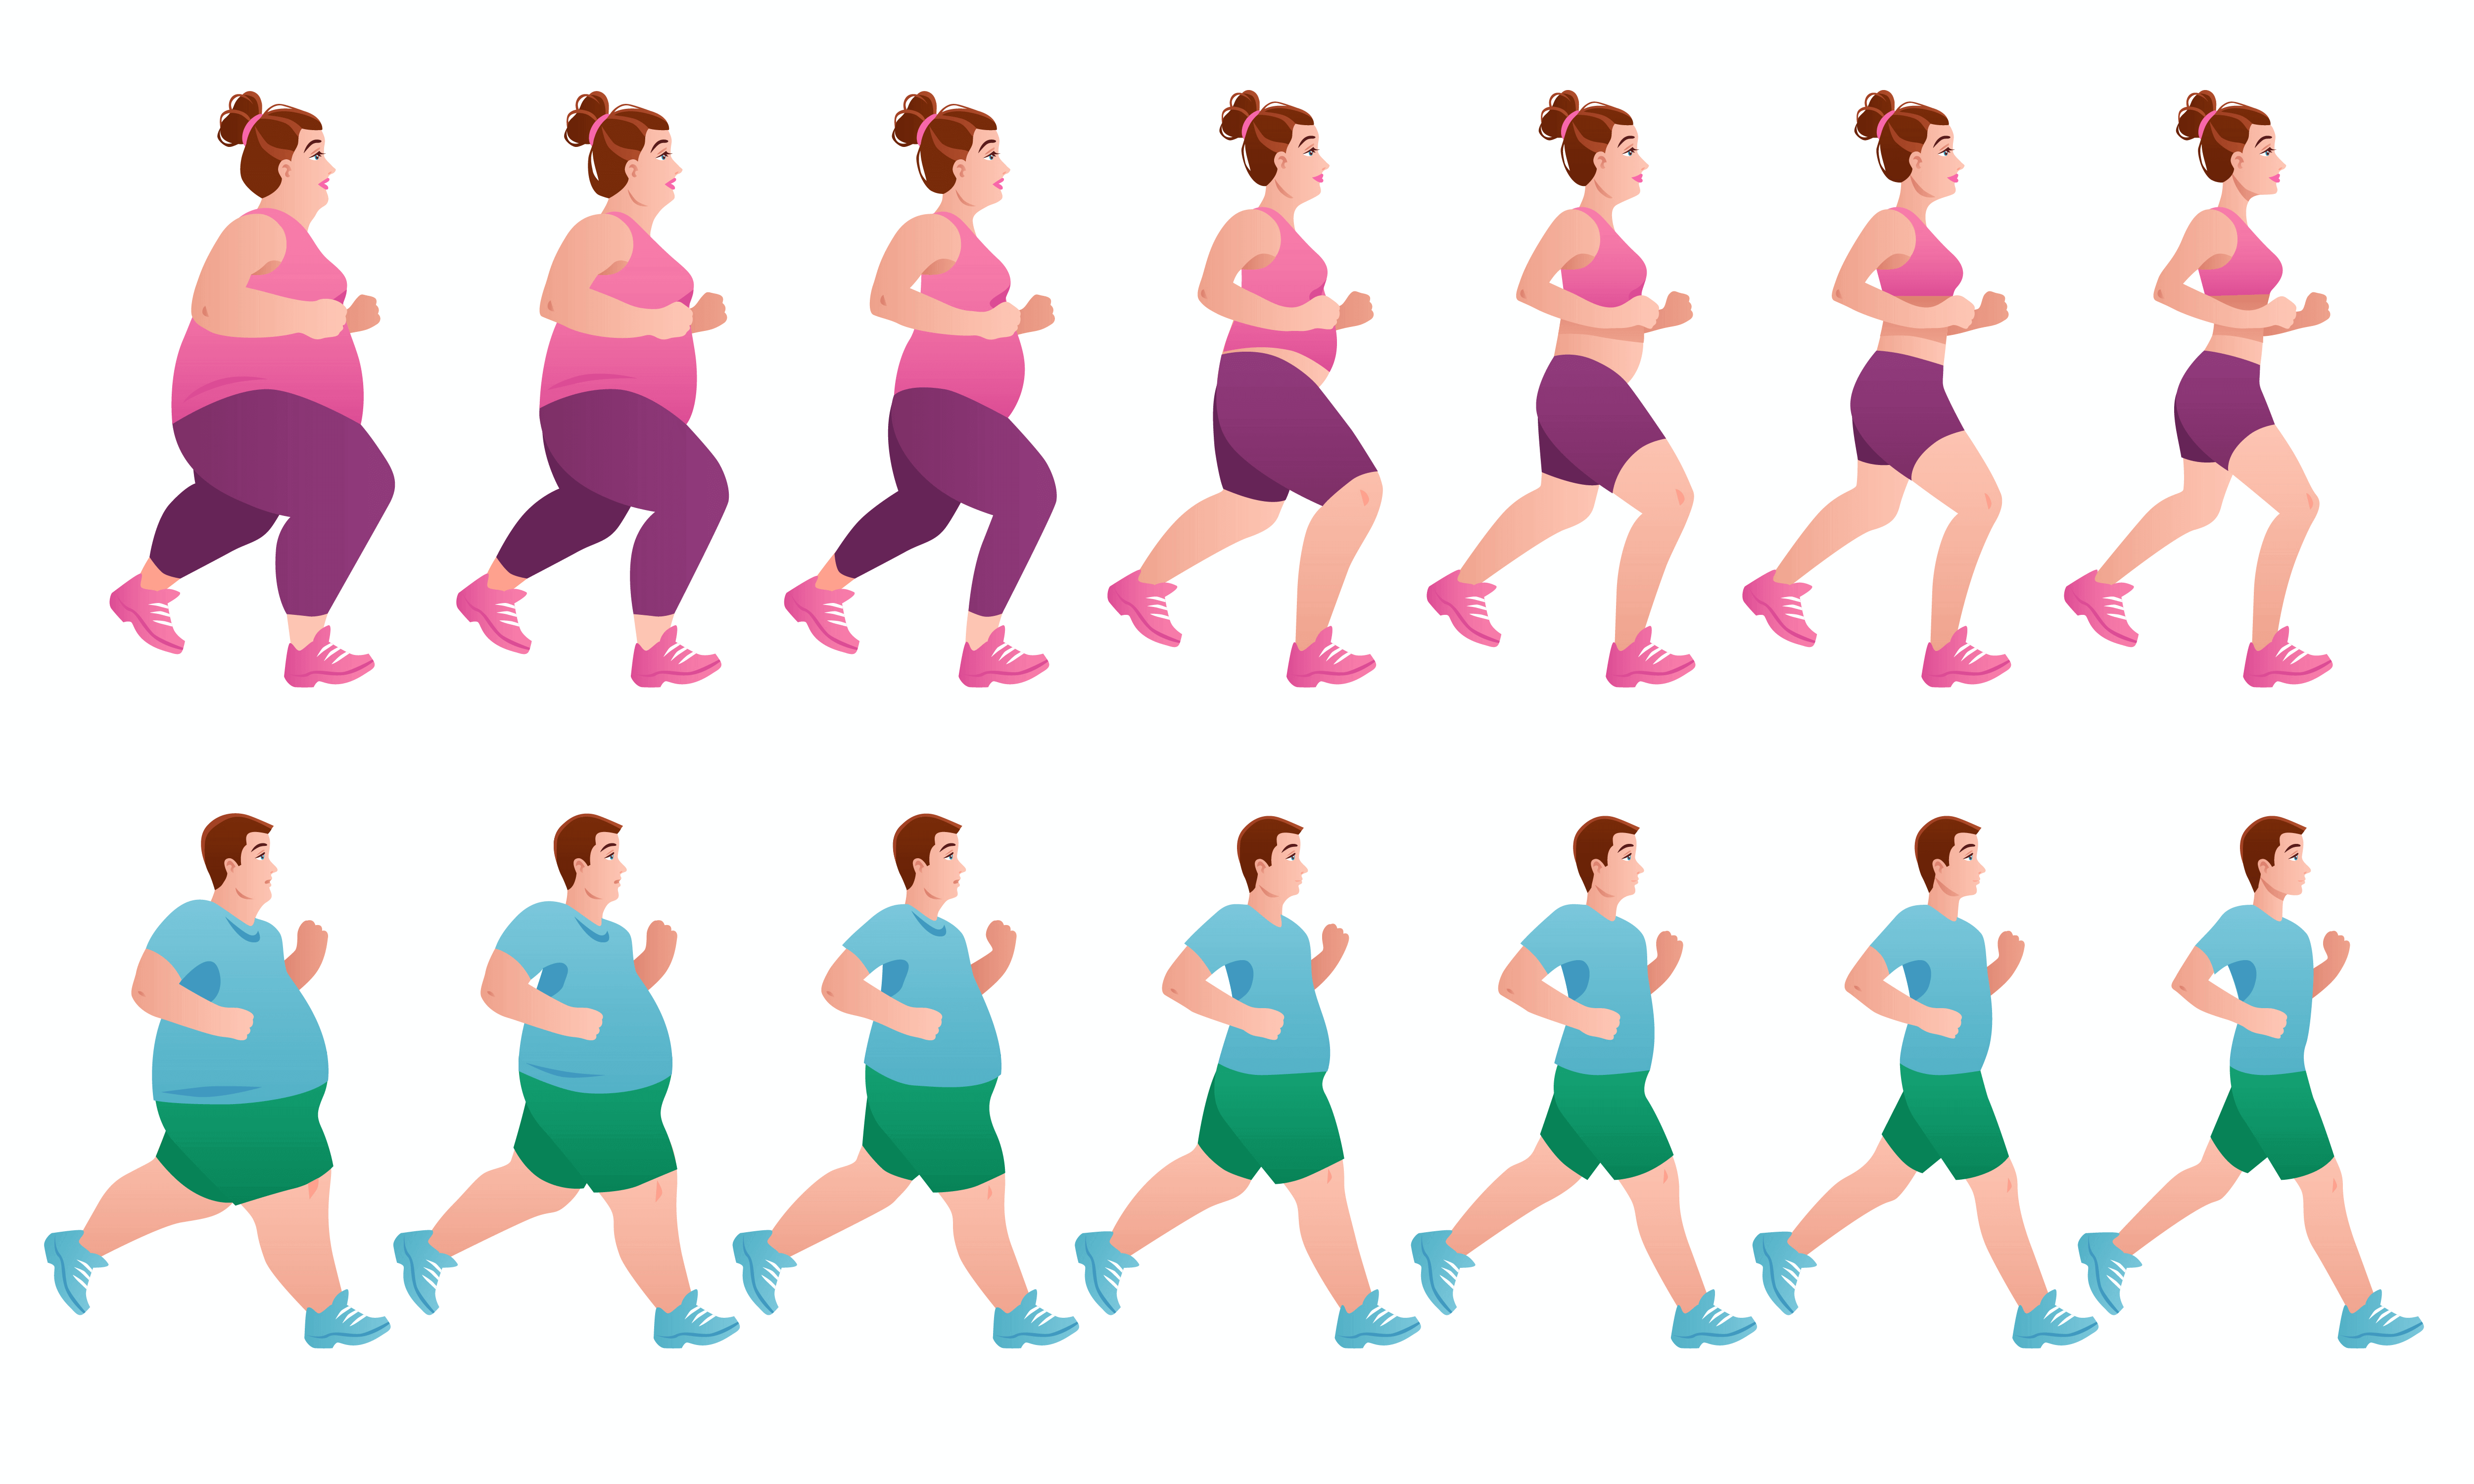
\includegraphics[width=.75\textwidth]{Images/NewIdeas/ExerciseTransformation.png}
    \caption{Example of how the virtual character could evolve as a result of training.}
    \label{fig:player_evolement}
\end{figure}

To register when the players are positioned at locations where they should earn points, geofencing will be used. Geofencing is based on defining areas on the map (illustrated in Figure \ref{fig:geofence}) where one can check whether or not the player is inside \citep{rouse_what_2016}. If the GPS location corresponds to a spot within the area, the player will be awarded points.

\begin{figure}[H]
    \centering
    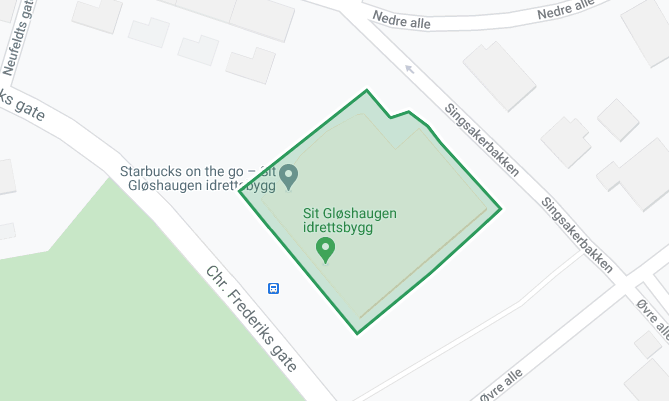
\includegraphics[width=.6\textwidth]{Images/NewIdeas/GeofenceExample.png}
    \caption{A geofence surrounding Sit Gløshaugen training center in Trondheim.}
    \label{fig:geofence}
\end{figure}

\textbf{Evaluation} \\
Hover is equivalent to Hold, categorized as an alternative game primarily based on  two reasons: Exploring alternative games variants by using gamification and using location data (GPS) as input in the gameplay.

The idea tries to increase people's well-being by motivating people to improve health, mental capabilities, socialize, and more. If the game concept is successful, it is valuable for both society and the individual.

Another important aspect when evaluating the concept is testability. Hover is easy to test because it has an extensive target group. Everyone owning a smartphone is a potential test subject. In addition to this, we think it will be easy to get people who agree to test this application because minimal extra time (despite answering a questionnaire) is required.

\subsection{Guess Where}
Guess Where is a challenge game, where players get to test how well they know their city. To earn points, players have to solve the challenges presented. A challenge consists of a street view picture where the player needs to figure out at which location it is captured; see Figure \ref{fig:street_view}). To complete the challenge, players must navigate to the correct site where their position is verified using GPS. The game is intended to reward completed challenges with fun facts about the area and in-game points.

\begin{wrapfigure}{r}{0.45\textwidth}
    \vspace*{-0.5\baselineskip}
    \centering
    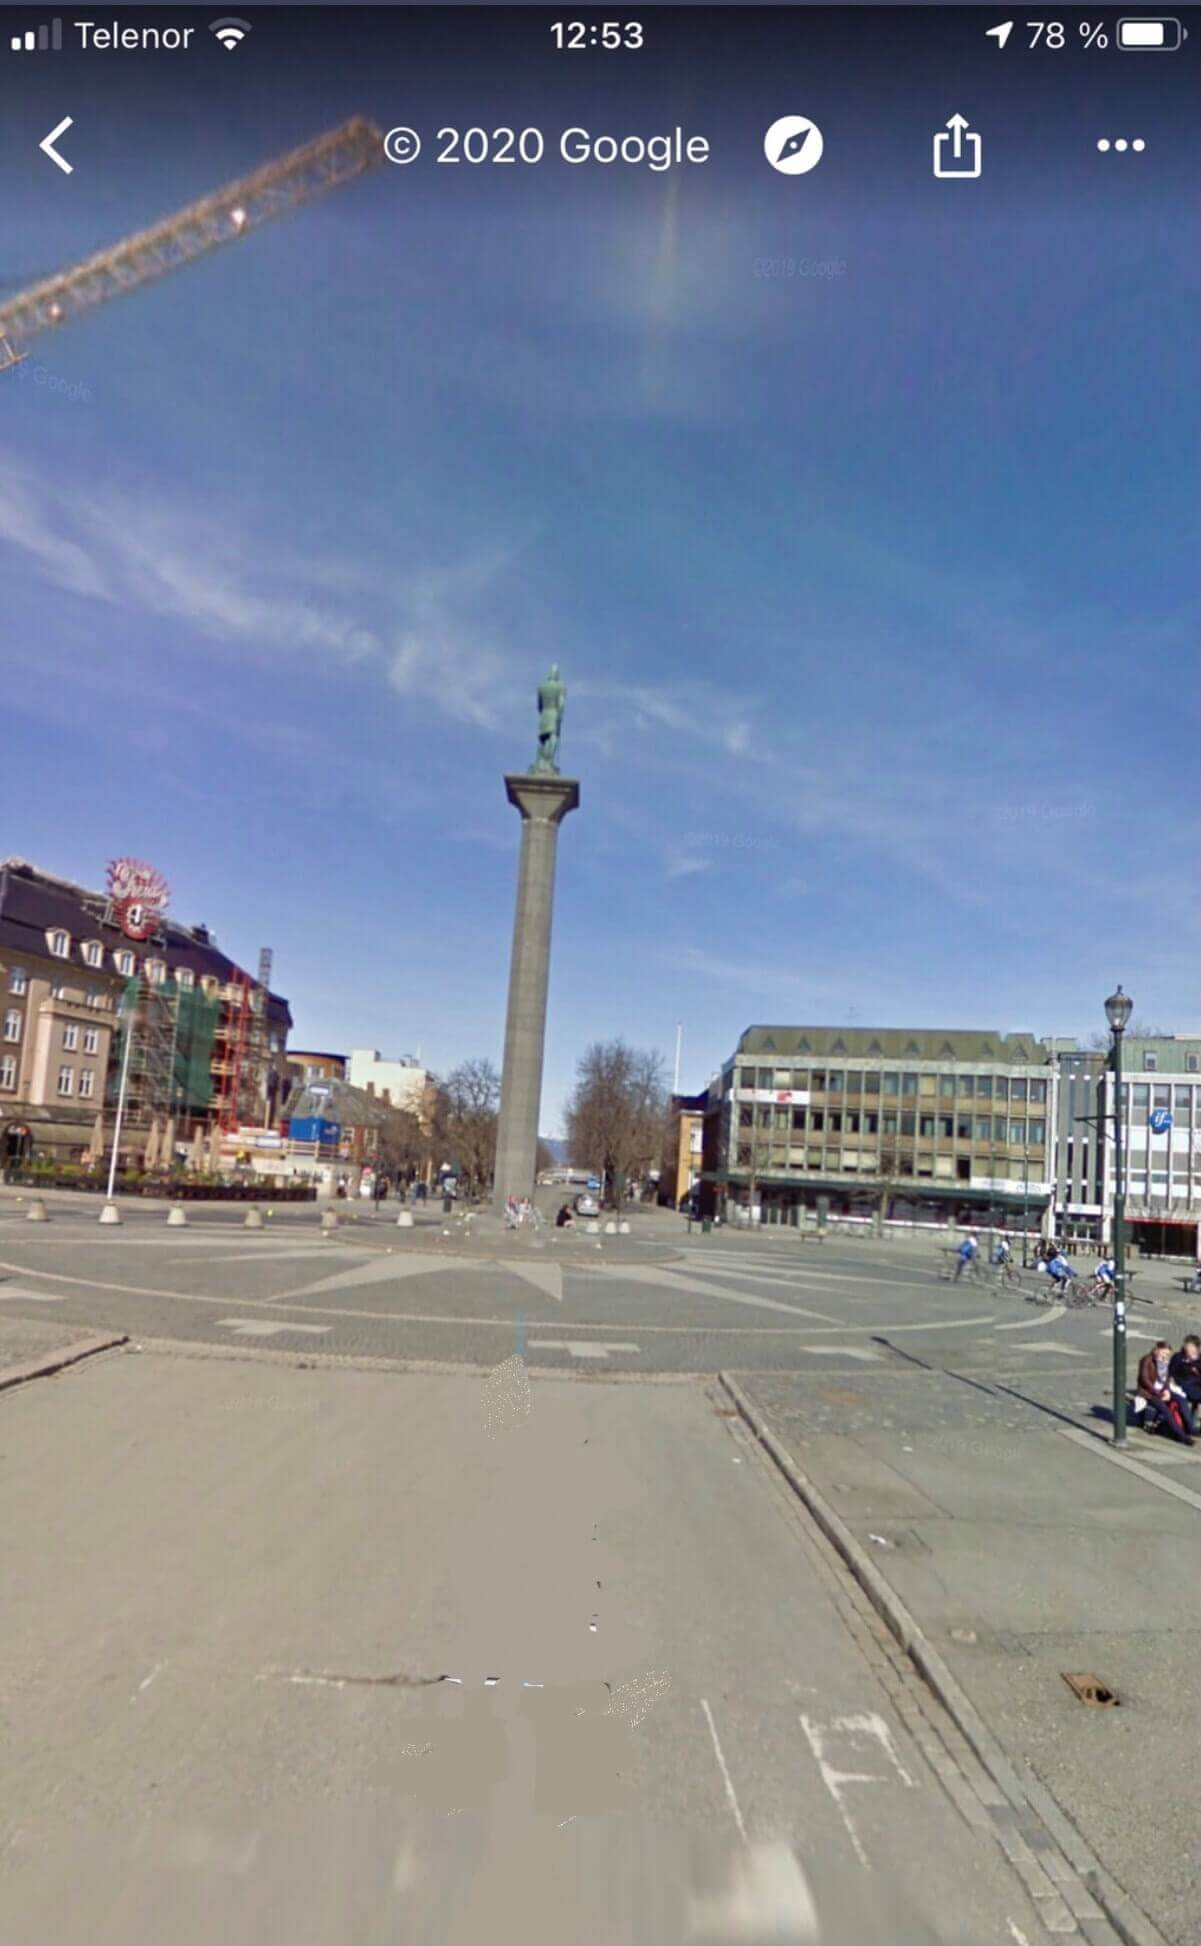
\includegraphics[width=0.35\textwidth]{Images/NewIdeas/StreetView.jpg}
    \caption{A street view photo of Trondheim Torg used as a hint in Guess Where.}
    \label{fig:street_view}
    \vspace*{-0.5\baselineskip}
\end{wrapfigure}

The concept can allow social interaction, both in the game and the real world. Players are encouraged to team up to boost their points. Accomplishments can also be shared with friends in a social feed inside the application. Social interaction through likes and comments can be motivating for further use. The concept is excellent for people that already have some knowledge of the city. However, by enabling hints, players can more easily complete the challenges.

\textbf{Evaluation}  \\
The concept fits into the alternative game model for several reasons, one being that the game is pervasive because it extends to the real world. As input, the game utilizes GPS for verifying a player’s location. In addition to this, the game fits into the domain of both entertainment and education. The game can also be categorized as gamification in the game variant category. 

The game concept is socially beneficial because it encourages social activities in the form of physical movement and collaboration while players can get to know the area better. One example where the game could be helpful is for educational purposes. Teenagers could team up and use this game for orientation in their gym classes. This approach could lead to improving cooperation skills while getting to know the city better. In terms of testability, this concept could easily, as in the example, be tested in a school class.

\subsection{Puzzle With Friends}
Puzzle With Friends is a game concept where the goal is to complete a puzzle together with your friends, as illustrated in Figure \ref{fig:friends_puzzle}. Each player is responsible for one piece they can move using their real-world position and rotating their mobile phone. All participants can watch the other players’ positions and the pattern they are supposed to puzzle in the application. The goal is to complete the puzzle, fit all the pieces in the correct spot, and rotate them correctly before the time is up. The number of pieces depends on how many players are collaborating on the same puzzle. Eight friends mean eight pieces, and so on. Thus the game will become increasingly challenging as the number of players increases. For the game to not become too easy, there should probably be a limitation on the minimum amount of players.

\begin{figure}[H]
    \centering
    \includegraphics[width=0.58\textwidth]{Images/NewIdeas/TeamworkPuzzleWithFriends.jpg}
    \caption{People collaborating to try to solve a puzzle in Puzzle With Friends.}
    \label{fig:friends_puzzle}
\end{figure}

GPS location will be used to determine the player’s position. Because of the limitation in GPS accuracy \citep{merry_smartphone_2019}, a large outdoor area is required for the game to work as intended. Parks or football fields are good examples. Also, the more players that are included in the game, the more space is needed. Hence, there probably should exist a maximum number of players per game. The gameplay should also have a suitable mechanism for “snapping” pieces into the correct place when they are almost correctly aligned. This tool will make the game more delightful to play when minor location errors are present.

\begin{wrapfigure}{r}{0.4\textwidth}
    \centering
    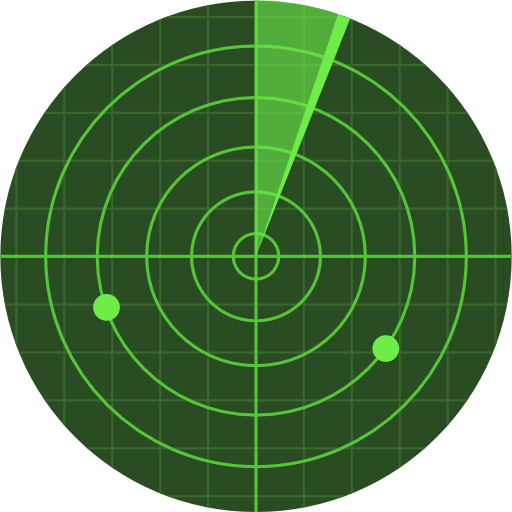
\includegraphics[width=0.35\textwidth]{Images/NewIdeas/Radar.png}
    \caption{A typical radar view. The “dots” will update every time the beam passes by.}
    \label{fig:radar_view}
    \vspace*{-1\baselineskip}
\end{wrapfigure}

As there probably will be some delay between the player’s movement and the application’s view, the gameplay needs to introduce some mechanism to hide this. One way to do this is by introducing some sort of radar view, see Figure \ref{fig:radar_view}, to illustrate that the other players’ position will only update at regular time intervals. 

\textbf{Evaluation}  \\
Puzzle With Friends is a typical alternative game because it uses alternative inputs to create a unique game concept. By utilizing the player’s position and heading in the real world to control the gameplay, the game is differentiated from other well-known puzzle games.

Developing the game should be manageable in the limited time we have during our master’s project. However, as mentioned above, inaccurate location data and real-time requirements may cause issues if not handled appropriately. Testing the application should be easy as long as we find some volunteers who agree to devote some hours of their day to test the application.

\subsection{Challenge Accepted}
Challenge Accepted is a social game that mixes social interaction with playful actions in the real world. The idea is based on a verbal game, often played among youths, called “\href{https://www.wikihow.com/Play-What-Are-the-Odds}{What are the odds?}”. The game is usually played between two players where one player (A) gives the dare, and another player (B) receives it. The challenges often occur in the moment, for instance, “What are the odds of you asking that stranger to try his crutches?” To extend the concept a bit, players can publish challenges on a location that pops up when their friends walk by.

\begin{figure}[H]
    \centering
    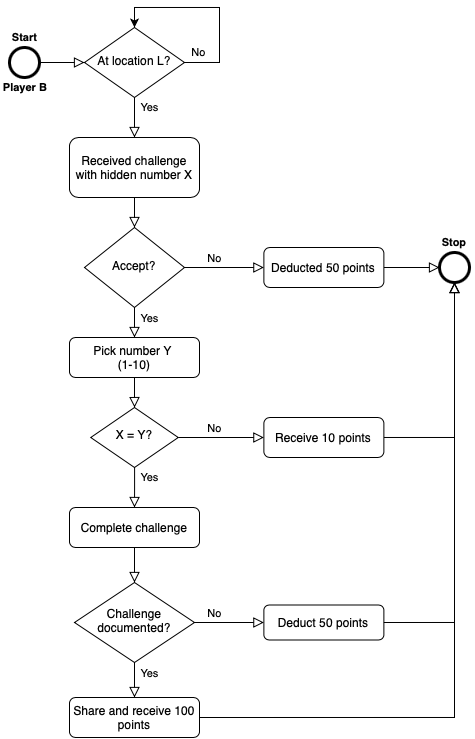
\includegraphics[width=.5\textwidth]{Images/NewIdeas/ChallengeAccepted.png}
    \caption{Flow chart illustrating a simplified game flow in Challenge Accepted.}
    \label{fig:challenge_accepted}
\end{figure}

Figure \ref{fig:challenge_accepted} shows a simplified game flow. The diagram is based on the following scenario: 

\begin{itemize}
    \item Player A adds a challenge to a location L, along with a number X between 1 and 10.
    \item A friend of player A, player B, walks by the location and receives a push notification.
    \item Player B has to either decline or accept the challenge. If the player chooses to decline, 50 points are lost. If the challenge is accepted, player B has to guess a number between 1 and 10.
    \item If the numbers are different, the player will not need to complete the challenge and receive 10 points for being courageous.
    \item However, if the numbers are equal, player B needs to do it. The challenge is considered completed when it is documented and shared in the application.
\end{itemize}

The goal of the game is to create spontaneous and surprising enjoyment between friends. The range of odds is set 1-10 because the risk of having to complete a challenge should not be too high nor too low. Also, challenges should be moderated to prevent them from being harmful. The game should include social interaction through likes and comments on in-game posts. Players should also be able to see their friends' game statistics and medals. Both these design elements are likely to have a positive effect on the competitiveness among friends.

\textbf{Evaluation}  \\
The idea classifies as alternative in the categories of input, game variant, and interaction. Besides location tracking, the concept also utilizes the camera for documenting challenges. Though the game is based on a verbal game, the game categorizes as gamification because players can be motivated through likes and comments on recent activities. 

The game is a pervasive game that utilizes location-tracking to create a bond between the virtual and the real world. The use of constant tracking of location contributes to the suspense of not knowing when, where, and what the next challenge will be. This suspense can also increase the players’ curiosity, and therefore their willingness to participate. 

The concept does not necessarily benefit society directly. However, it is a social game that has value for a smaller group of people. For testing purposes, it is advantageous to test the game on people with a pre-existing relationship, to enhance the players’ motivation to complete the challenges.

\subsection{Secret Posts}
Secret Posts is an extension and gamification concept based on the social app \href{https://jodel.com}{Jodel}, where players can share anonymous posts in their city. Since the posts are anonymous, people tend to post their secrets, embarrassing stories, and pictures. Our concept involves posting digital notes, drawings, or images in the real world, which only can be seen using Augmented Reality (AR) technology. All players can share posts attached to the location where they are posted. An example can be a sticky-note with a secret message lying on a table in a cafeteria. To find posts, players use a map to locate nearby ones, as seen in Figure \ref{fig:secret_notes_map}. Although the posts’ location is visible on the map, the content is only available through the mobile camera. As illustrated in Figure \ref{fig:secret_notes_camera}, players use their mobile camera to read new posts in their current area. Since the posts only are visible to the players, a secret society is created where “only those who know, know.”

\begin{figure}[H]
    \begin{minipage}{.48\textwidth}
        \centering
        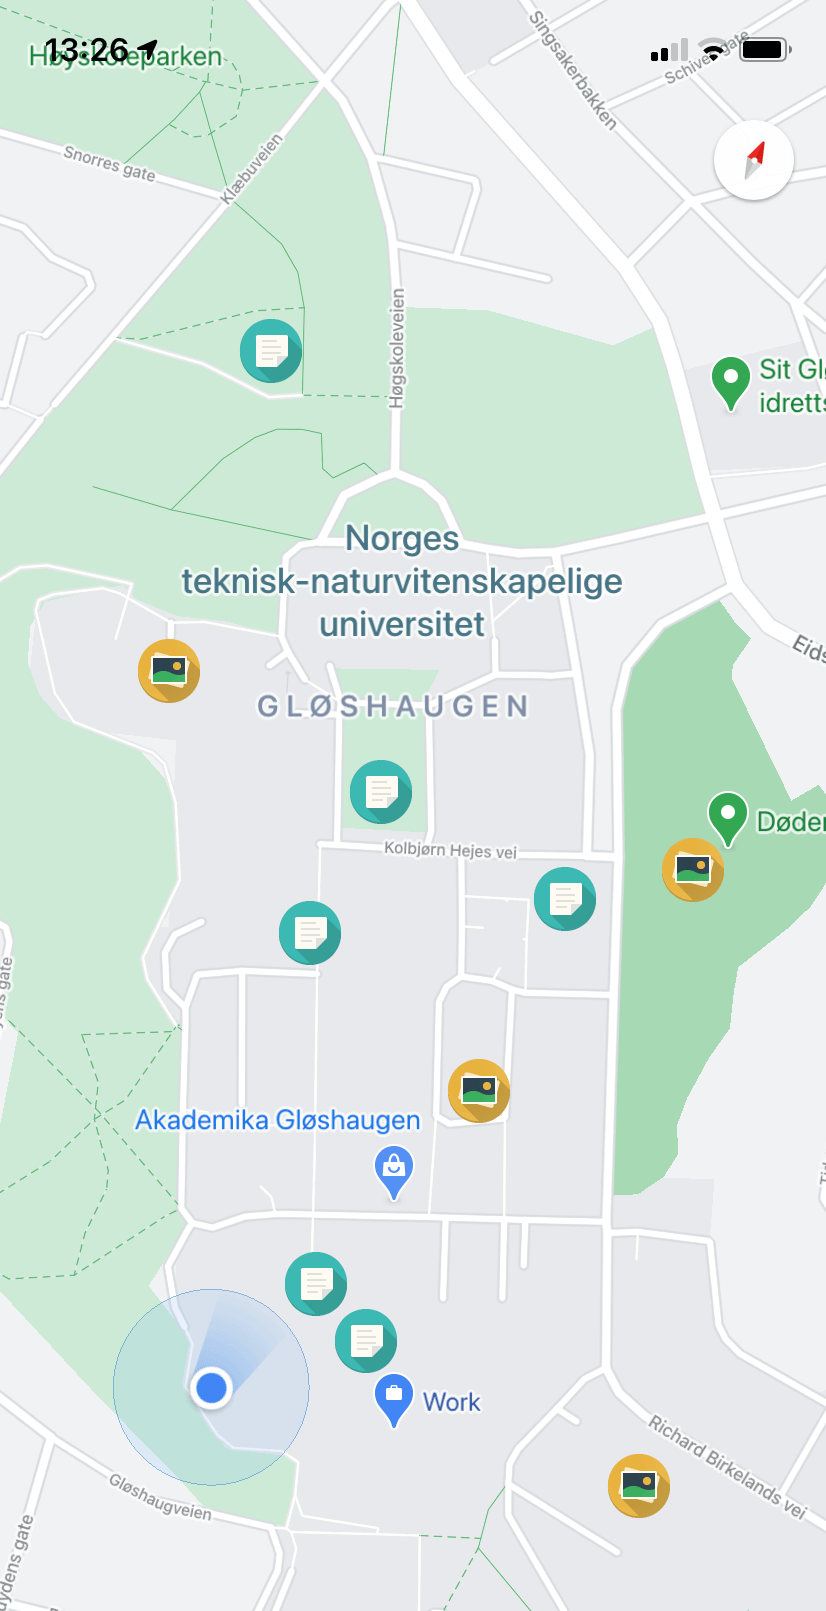
\includegraphics[width=.8\textwidth]{Images/NewIdeas/SecretNotesMap.png}
        \captionof{figure}{The map-view in Secret Notes showing nearby posts.}
        \label{fig:secret_notes_map}
        \end{minipage}
        \hspace*{0.5\baselineskip}
        \begin{minipage}{.48\textwidth}
        \centering
        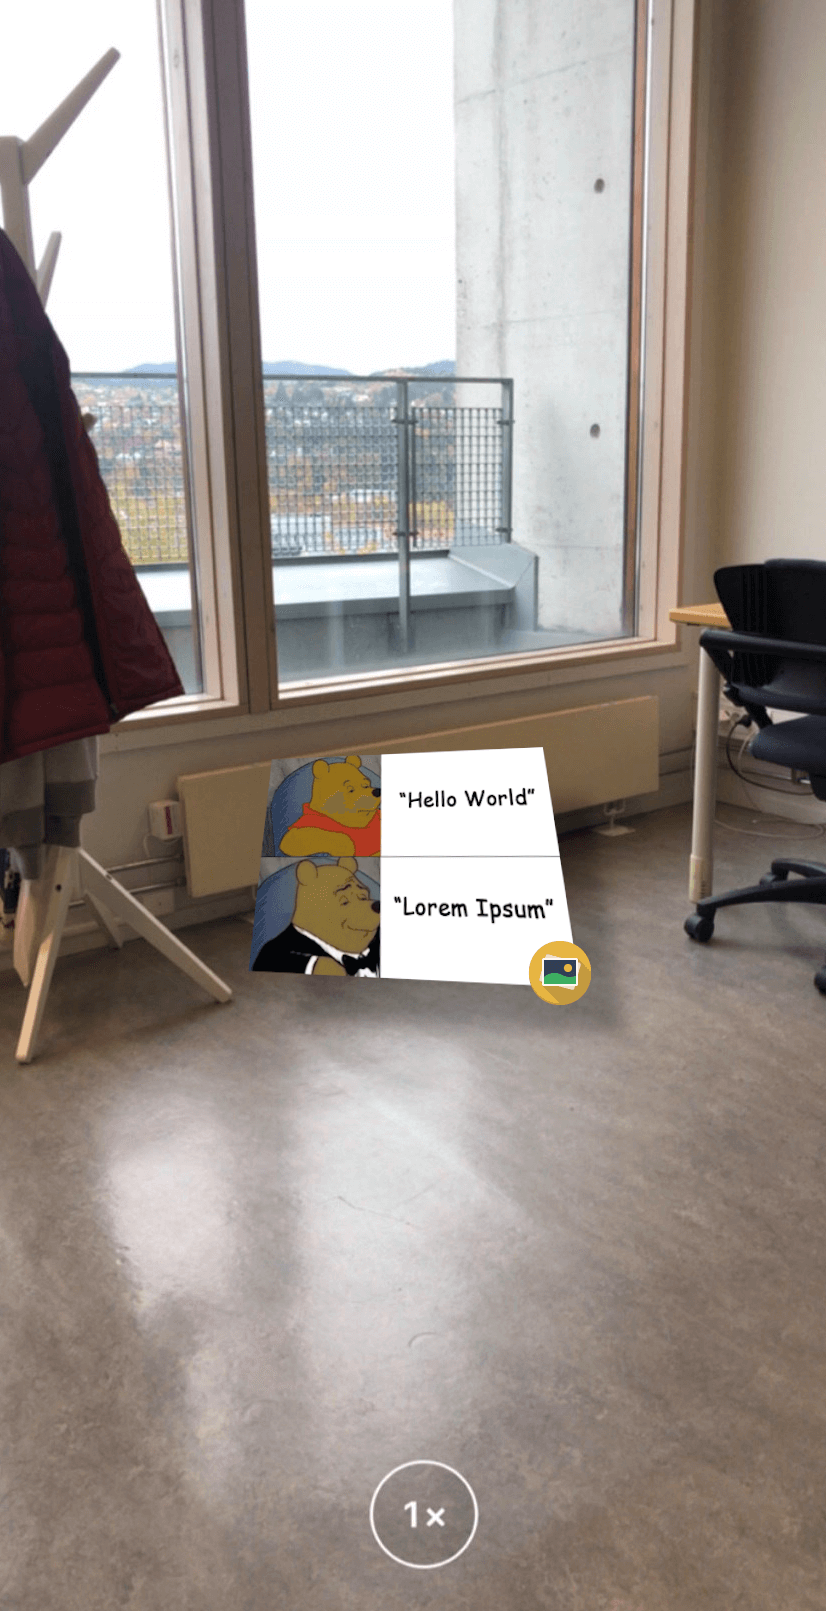
\includegraphics[width=.8\textwidth]{Images/NewIdeas/SecretNotesCamera.png}
        \captionof{figure}{AR view of the content of a note found in Secret Notes.}
        \label{fig:secret_notes_camera}
    \end{minipage}
\end{figure}

\textbf{Evaluation}  \\
The concept is alternative in its usage of input, output, game genre, and concept. The game uses the phone’s camera as input, which it uses to project a note, image, or drawing. This usage of AR is not too common as of 2021; hence the input method is alternative. The concept is also alternative because it uses location to attach anonymous posts. Tangible objects like notes, posters, and graffiti are not unfamiliar in the real world. However, the fact that the posts are only visible for those who search for them makes the game alternative.

The concept is suited for AR glasses and as a mobile application. The benefit of using AR glasses is that the users can walk around and discover notes without actively looking. However, in terms of testability, the AR glasses approach has a clear disadvantage compared to a mobile application in terms of equipment available and the project’s time scope. As a mobile application, the concept should be straightforward to develop and test.

\subsection{Free Ticket to Ride}
The purpose of this game concept is to incentivize having a valid ticket when using public transport. The idea is to create an application that gamifies the ticket system used on public transport. It could be adopted as an alternative or addition to normal ticket controls used today.

The application will need to integrate with the existing application to validate tickets. People who have paid for a valid ticket will be given points in the game when traveling. After earning a set amount of points, the user can “purchase” free items or get discounts. One suggestion is to use free or discounted single tickets as rewards. For example, twenty rides with a valid ticket could qualify for one free ticket. A prerequisite for this is, of course, a partnership with a public transport company, such as AtB in Trondheim. Even though the concept is invented and conceptualized based on the public transport system in Trondheim, the same ideas could be adopted in other cities with similar ticket systems as well.

The application can communicate with a Bluetooth access point to check if a user is located in a public transport vehicle and award points accordingly (illustrated in Figure \ref{fig:people_on_the_bus}). A secondary registration option using the camera and scanning QR codes could also be an alternative to situations where the bus does not have a Bluetooth access point, or the user does not consent to Bluetooth usage.

\begin{figure}[H]
    \centering
    
\includegraphics[width=0.75\textwidth]{Images/NewIdeas/PeopleOnTheBus.png}
    \caption{Illustration of people using Free Ticket to Ride on public transport.}
    \label{fig:people_on_the_bus}
\end{figure}

\textbf{Evaluation}  \\
Free ticket to ride is an alternative game concept because it uses Bluetooth as input. Additionally, the idea explores the gamification variant. By the definition of an alternative game (Chapter \ref{chap:what_is_alternative_game}), exploring theses two categories of characteristics define this as alternative.

The game introduces a fun way of validating the user’s ticket when using public transport, which could lead to fewer fare evasions. Getting more people to pay for their ride will result in more income for the public transport company, which can improve the service. 

One of the main problems with this idea is the need for tight integration with the current public transport company. The concept requires integration with the ticket system to check the validity of the ticket.

\subsection{Comparison of Game Concepts}
Similarly, as in Chapter \ref{chap:comparison_of_existing_games}, when existing alternative game concepts were presented, our new ideas are compared using the alternative games model described in Chapter \ref{chap:design_an_enjoyable_game}. All of the game concepts are categorized using the model of alternative games.

In contrast to the comparison of existing alternative games, our new concepts have a lot in common and often tick the same boxes in the model, as seen in Table \ref{tab:new_ideas_comparison}. The existing alternative games were picked partly based on their difference, so this is expected. As mentioned at the beginning of this chapter, we limited ourselves to concepts based on the mobile platform. Thus all the games are restricted to input and output provided by a smartphone. For input, a selection of the available sensors in a mobile phone has been used. GPS for location tracking is the most common, with four out of six concepts using it. Output possibilities on a mobile phone are more limited. There are not a lot of possible outputs that we would categorize as alternative. Two exceptions are found in Secret Posts and Free Ticket to Ride. These games respectively use an AR screen for displaying the notes and SMS to verify users and notify them of important events.

\begin{table}[H]
    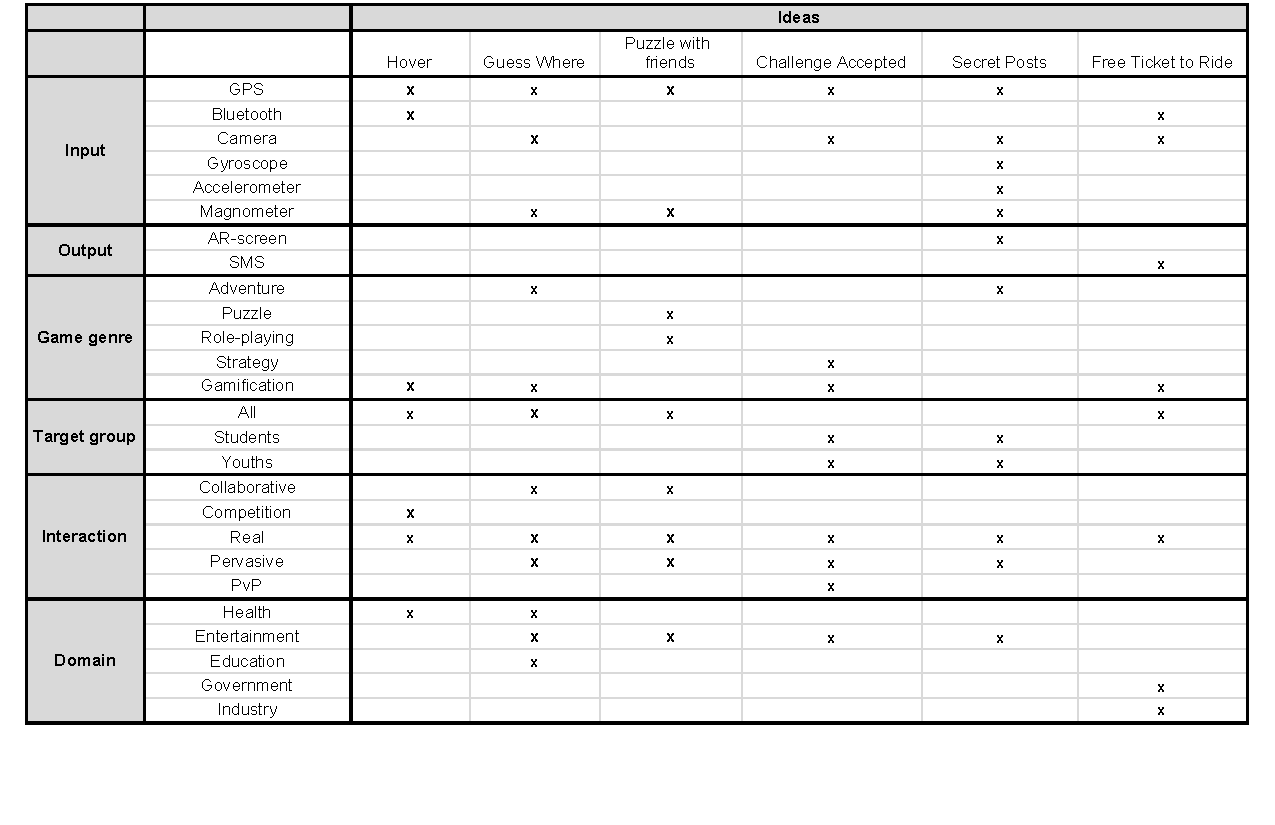
\includegraphics[width=1\textwidth]{Images/Models/OurConcepts.pdf}
    \vspace*{-1\baselineskip}
    \caption{Comparison of Game Concepts}
   \label{tab:new_ideas_comparison}
\end{table}

One of the most notable similarities in the comparison is the use of gamification as the game variant. This similarity is related to our goal in the project; trying to do something socially beneficial. We found it easier to invent gamification ideas with a socially beneficial purpose than other game variants.

As we also described in our motivation (Chapter \ref{chap:motivation}), an influential factor when inventing ideas was trying to reach as many users as possible. Therefore, the applications are usually targeted at all user types. However, two of the concepts have youths and students as the primary target group.

The last two categories address interaction and domain. In the interaction category, we see that all games include aspects of the real-world. Four of the games are also pervasive, meaning that they mix reality and virtuality. The most common domain in the applications is entertainment, with four of six applications characterized as it. Hover and Free Ticket to Ride are the only ones that are not categorized as entertainment. They fall into the health and government/industry domain, respectively.

\subsection{Summary}
In this chapter, our ideas for new alternative game concepts were described. A brief description of all of the concepts and an evaluation of them were conducted. We looked at why the concepts can be categorized as alternative games and how they fit with our goal and motivation in the project. Additionally, we looked at the testability of the ideas. Last, we compared the concepts and looked at differences using the alternative games model defined earlier. The next chapter will use these observations and evaluations when we will choose the concept we are going to develop in our master’s thesis.
